\documentclass[12pt]{article}
\usepackage{geometry}                % See geometry.pdf to learn the layout options. There are lots.
\geometry{letterpaper}                   % ... or a4paper or a5paper or ... 
%\geometry{landscape}                % Activate for for rotated page geometry
\usepackage[parfill]{parskip}    % Activate to begin paragraphs with an empty line rather than an indent
\usepackage{daves,fancyhdr,natbib,graphicx,dcolumn,amsmath,lastpage,url}
\usepackage{amsmath,amssymb,epstopdf,longtable}
\usepackage{paralist} 
\usepackage[final]{pdfpages}
\DeclareGraphicsRule{.tif}{png}{.png}{`convert #1 `dirname #1`/`basename #1 .tif`.png}
\pagestyle{fancy}
\lhead{CE 3372 -- Water Systems Design}
%%%%%%%%%%%%%%%%%%%%%%%%%%%%%%
%%%%%%%%%%%%%%%%%%%%%%%%%%%%%%
%%%%%%%%%%%%%%%%%%%%%%%%%%%%%%
\rhead{FALL 2025}
\lfoot{EXERCISE 2}
\cfoot{}
\rfoot{Page \thepage\ of \pageref{LastPage}}
\renewcommand\headrulewidth{0pt}
%%%%%%%%%%%%%%%%%%%%%%%%%%%%%%%
%%%%%%%%%%%%%%%%%%%%%%%%%%%%%%%
%%%%%%%%%%%%%%%%%%%%%%%%%%%%%%%
\begin{document}
\begin{center}
{\textbf{{ CE 3372 -- Water Systems Design} \\ {Exercise 2}}}
\end{center}
\section*{\small{Purpose}}
\begin{itemize}
\item Demonstrate ability to summarize engineering literature, and communicating that summary in writing.
\end{itemize}
\begin{enumerate}

\item{\textbf{Los Angeles Aqueduct History}}
Read the attached article from a 2013 issue of ``Civil Engineering.''   Prepare a summary of the article.   In the summary describe the Los Angeles Aqueduct.  List the different types of conveyances and hydraulic machines that are employed (closed conduit, open conduit, lift stations, etc.) in its operation.  Explain what design and/or construction features were employed that were novel for their time.  Conclude with a comparison of the Los Angeles Aqueduct to a large-diameter gas pipeline.  What are the similarities and differences (other than the working fluid!).\footnote{This exercise supports General Program Outcome (g) ``an ability to communicate effectively'' and (h) ``the broad education necessary to understand the impact of engineering solutions in a global and societal context.''   This exercise is ``Writing Intensive.''}
\end{enumerate}
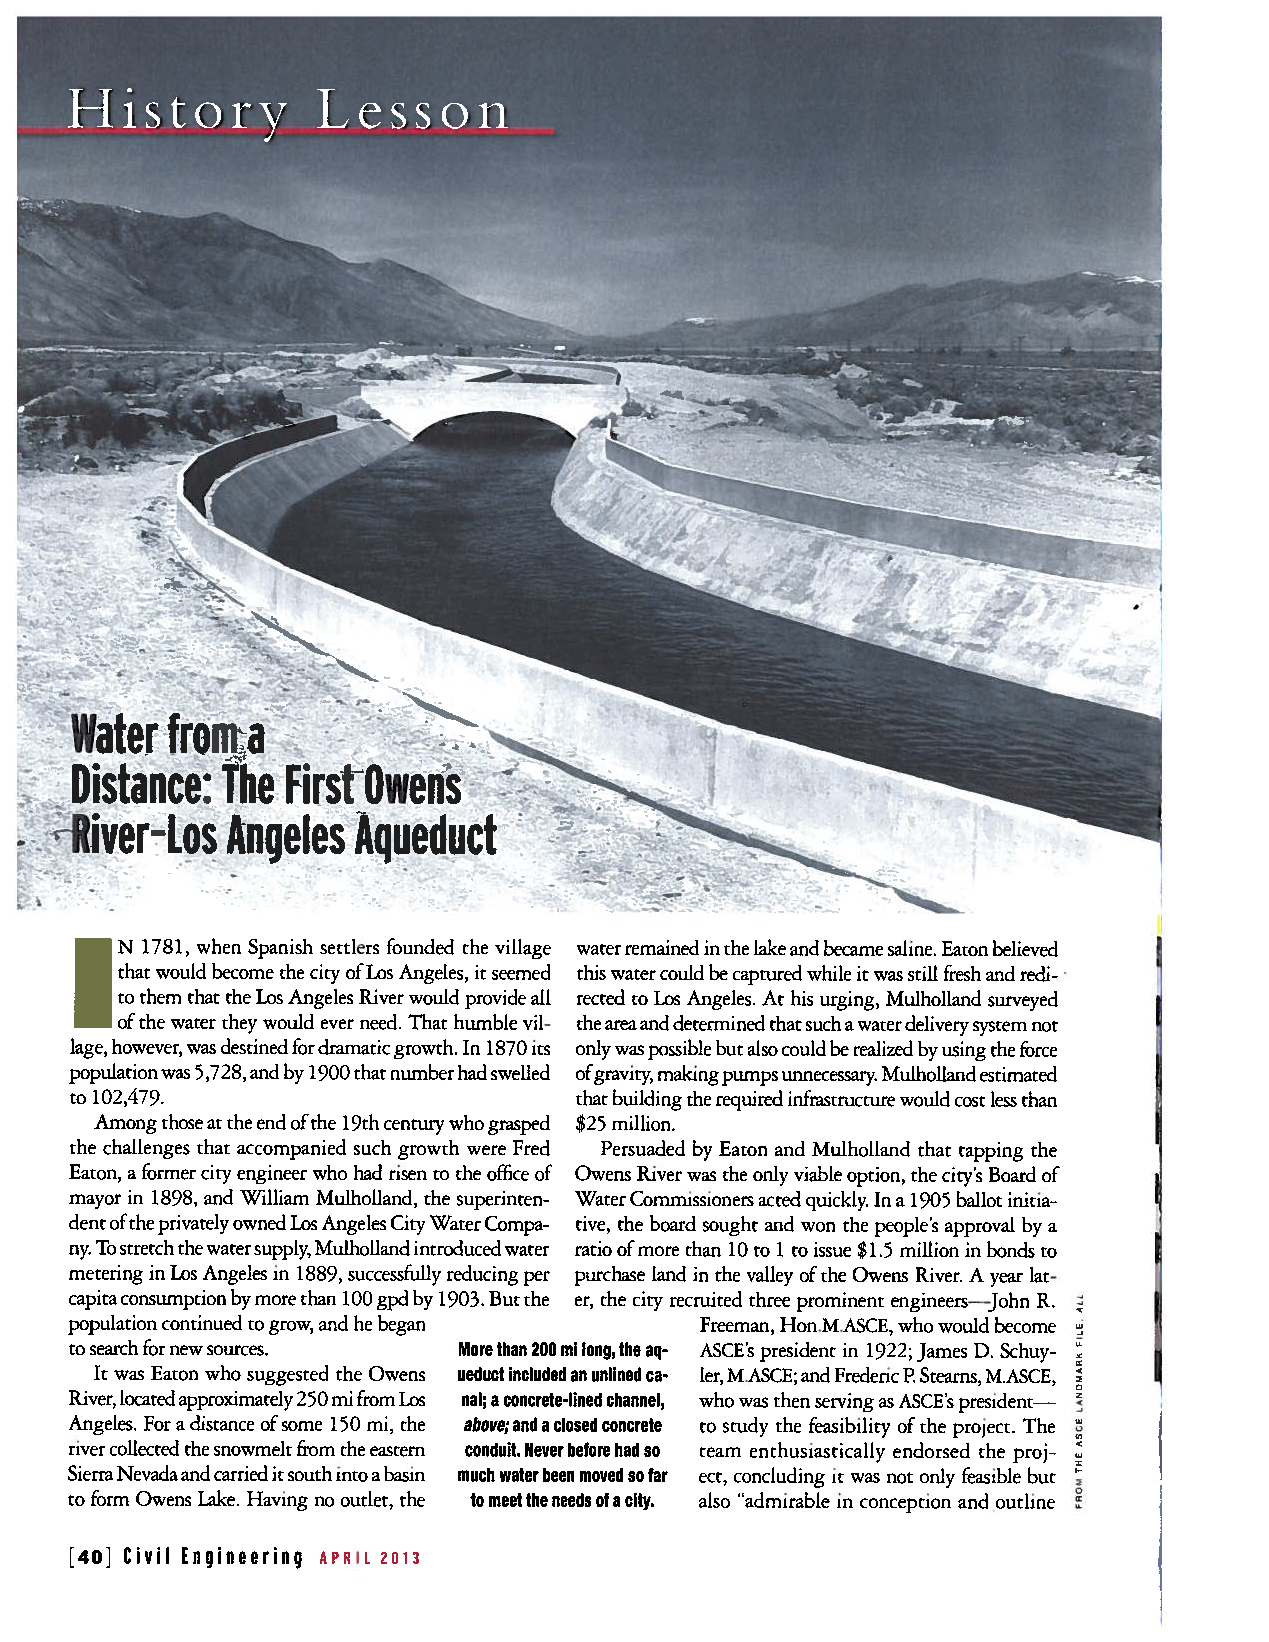
\includepdf[pages={-}]{./LosAngelesAquaductHistory.pdf}

\end{document}  